\documentclass[preview]{standalone}
\usepackage{tkz-graph}
\begin{document}

\begin{figure}[ht]
\center
 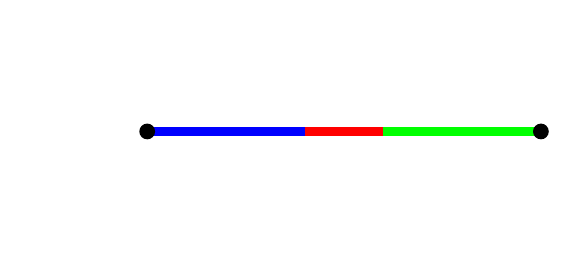
\begin{tikzpicture}
   \draw[color=white,line width=75pt] (-0.2,0) -- (-0.1,0);
   \draw[color=blue,line width=3pt] (0,0) -- (2,0);
   \draw[color=red,line width=3pt] (2,0) -- (3,0);
   \draw[color=green,line width=3pt] (3,0) -- (5,0);
   \fill [black] (0,0) circle (0.1);
   \fill [black] (5,0) circle (0.1);
 \end{tikzpicture}
\end{figure}

% \begin{figure}[ht]
% \center
%  \begin{tikzpicture}
%    \draw[color=white,line width=75pt] (-0.2,0) -- (-0.1,0);
%    \draw[color=blue,line width=3pt]  (0,0) to [out=45,in=180]  (3,-1);
%    \draw[color=red,line width=3pt]  (3,-1) to [out=0,in=180]  (5,0);
%    \fill [black] (0,0) circle (0.1);
%    \fill [black] (5,0) circle (0.1);
%  \end{tikzpicture}
% \end{figure}

% \begin{figure}[ht]
% \center
%  \begin{tikzpicture}
%    \draw[color=blue,line width=3pt]  (0,3) -- (3,4.5);
%    \draw[color=blue,line width=3pt]  (0,3) -- (6,4);
%    \draw[color=red,line width=3pt]  (0,3) -- (5,1);
%    \draw[color=green,line width=3pt]  (3,4.5) -- (5,1);
%    \draw[color=red,line width=3pt]  (3,4.5) -- (6,4);
%    \draw[color=blue,line width=3pt]  (6,4) -- (8,2);
%    \draw[color=green,line width=3pt]  (8,2) -- (5,1);
%    \fill [black] (0,3) circle (0.1);
%    \fill [black] (3,4.5) circle (0.1);
%    \fill [black] (6,4) circle (0.1);
%    \fill [black] (5,1) circle (0.1);
%    \fill [black] (8,2) circle (0.1);
%  \end{tikzpicture}
% \end{figure}

\end{document}



После: convert pdf to png
https://convertio.co/pdf-png/



 






